\chapter{Problem 1}

\section{Figure 1}

    \subsection{Histogram}

    \begin{figure}[h]
        \centering
        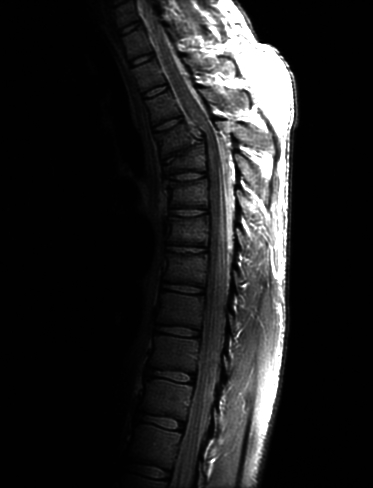
\includegraphics[width=\linewidth]{./images/Fig1.jpg}
        \caption{Fig1.jpg}
        \label{diagram:fig1}
    \end{figure}

    \begin{figure}[h]
        \centering
        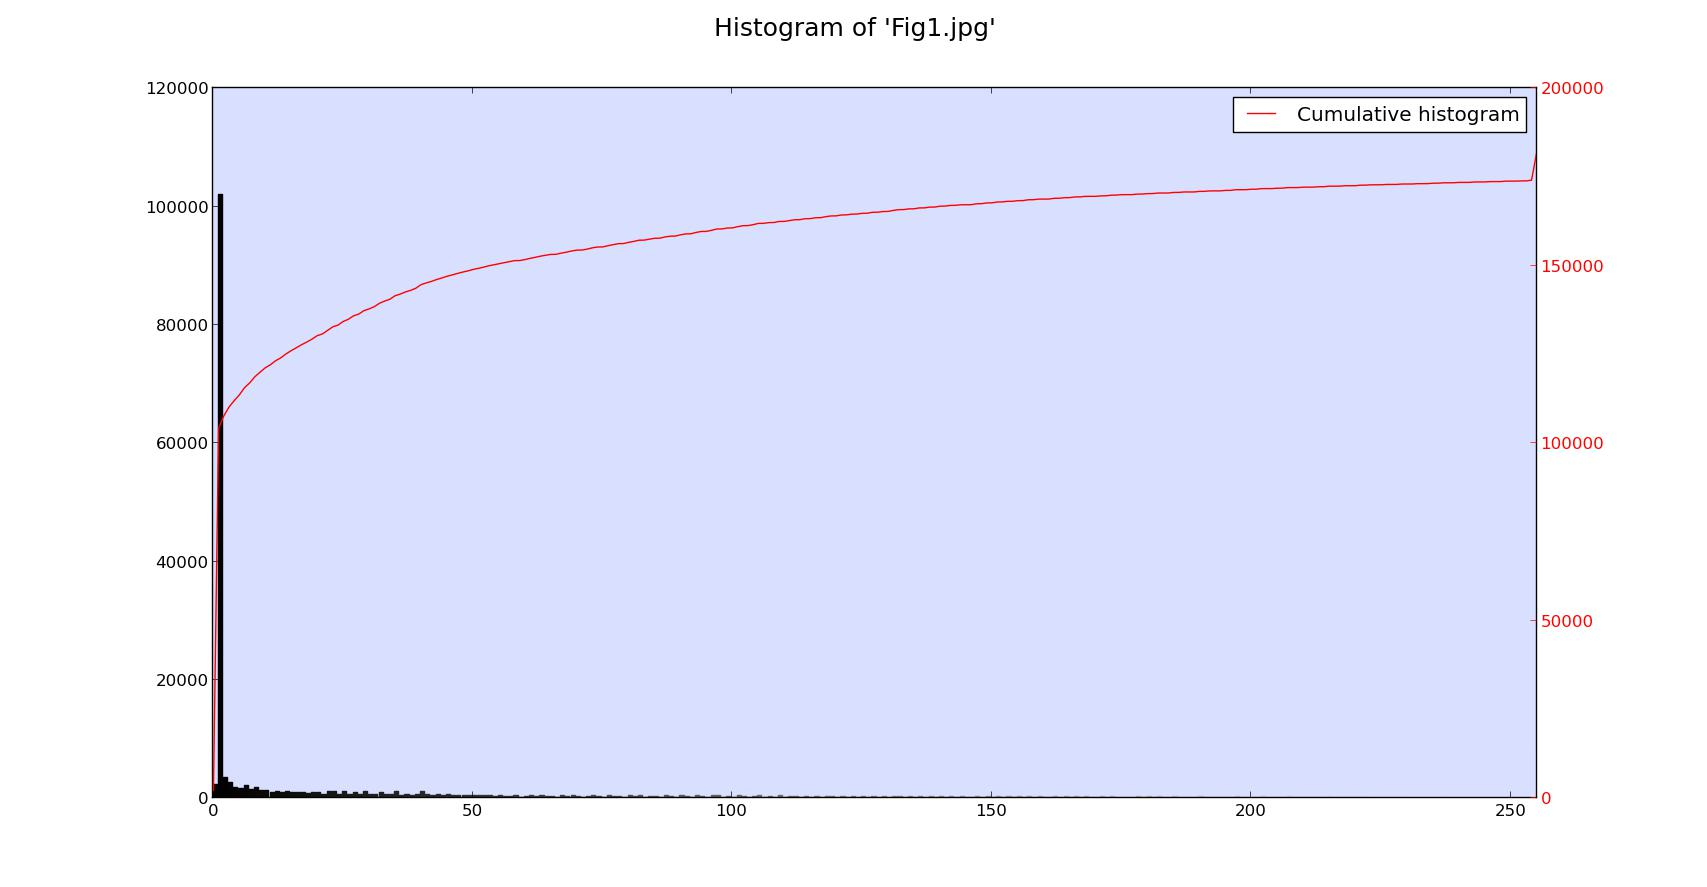
\includegraphics[width=\linewidth]{./images/Histogram_Fig1.jpg}
        \caption{Histogram of "Fig1.jpg"}
        \label{diagram:hist_fig1}
    \end{figure}

    \subsection{Histogram equalization}

    \begin{figure}[h]
        \centering
        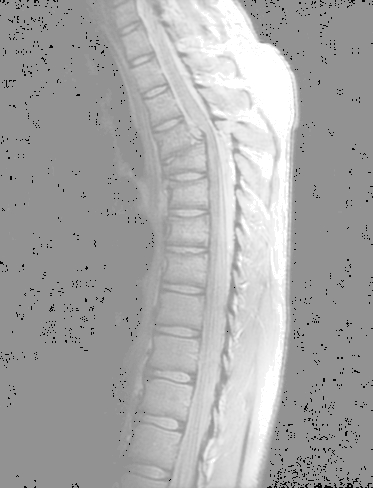
\includegraphics[width=\linewidth]{./images/Enhanced_Fig1.jpg}
        \caption{Enhanced Fig1.jpg}
        \label{diagram:enhanced_fig1}
    \end{figure}

    \begin{figure}[h]
        \centering
        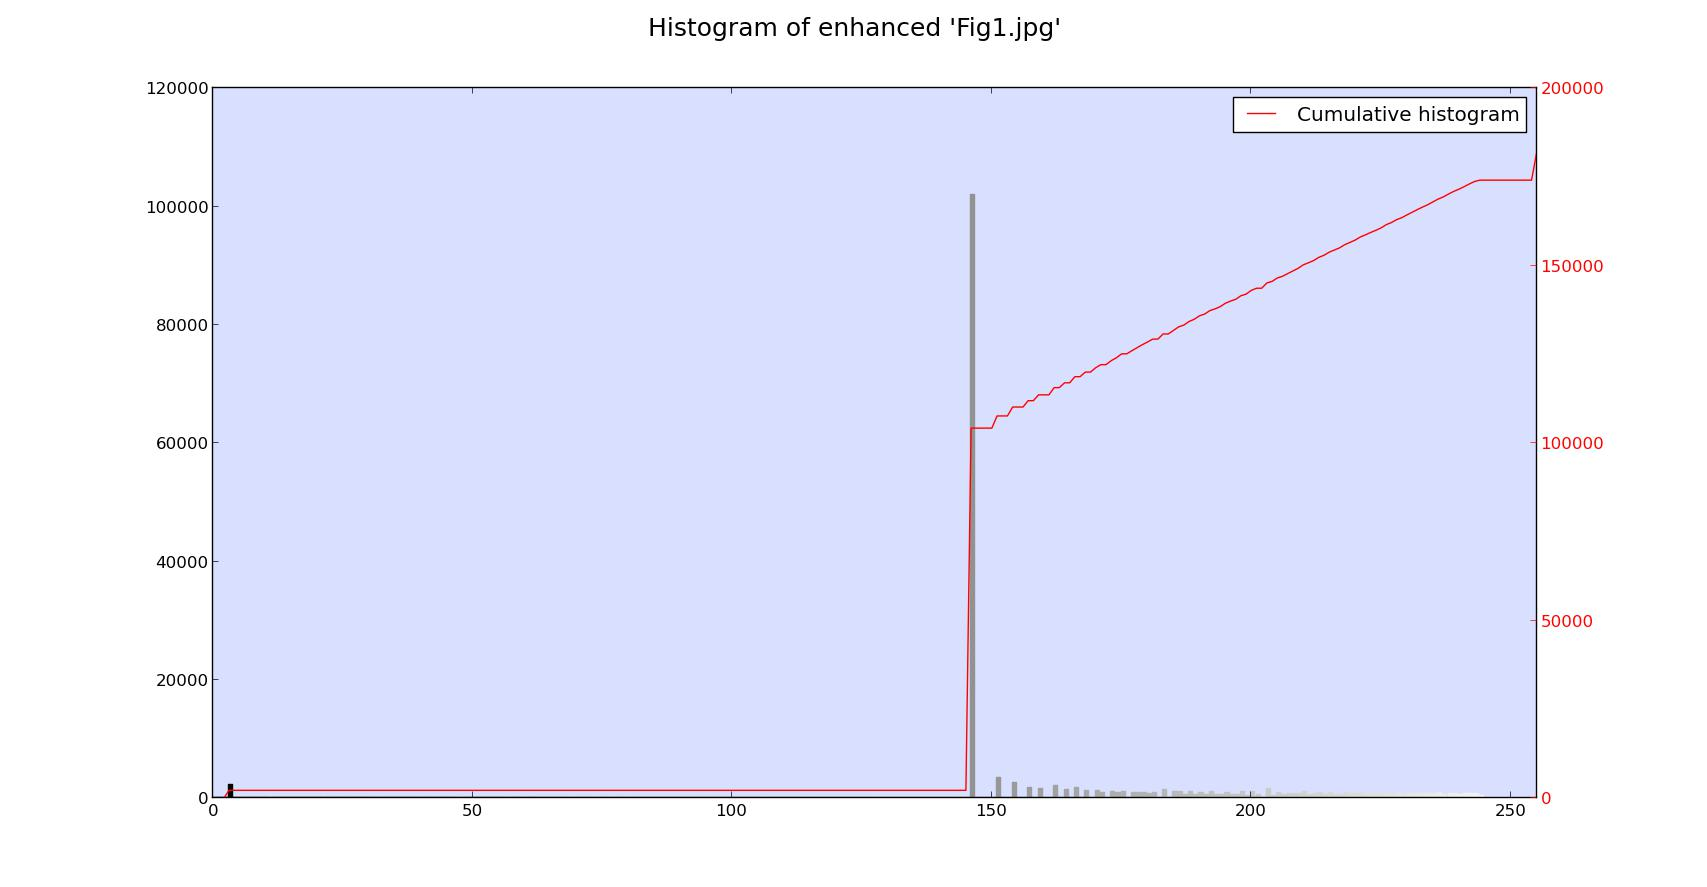
\includegraphics[width=\linewidth]{./images/Equalized_Histogram_Fig1.jpg}
        \caption{Equalized histogram of "Fig1.jpg"}
        \label{diagram:equal_hist_fig1}
    \end{figure}


\section{Figure 2}

    \subsection{Histogram}

    \begin{figure}[h]
        \centering
        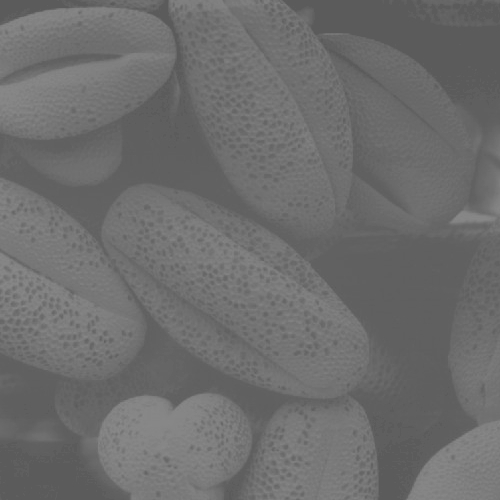
\includegraphics[width=\linewidth]{./images/Fig2.jpg}
        \caption{Fig1.jpg}
        \label{diagram:fig1}
    \end{figure}

    \begin{figure}[h]
        \centering
        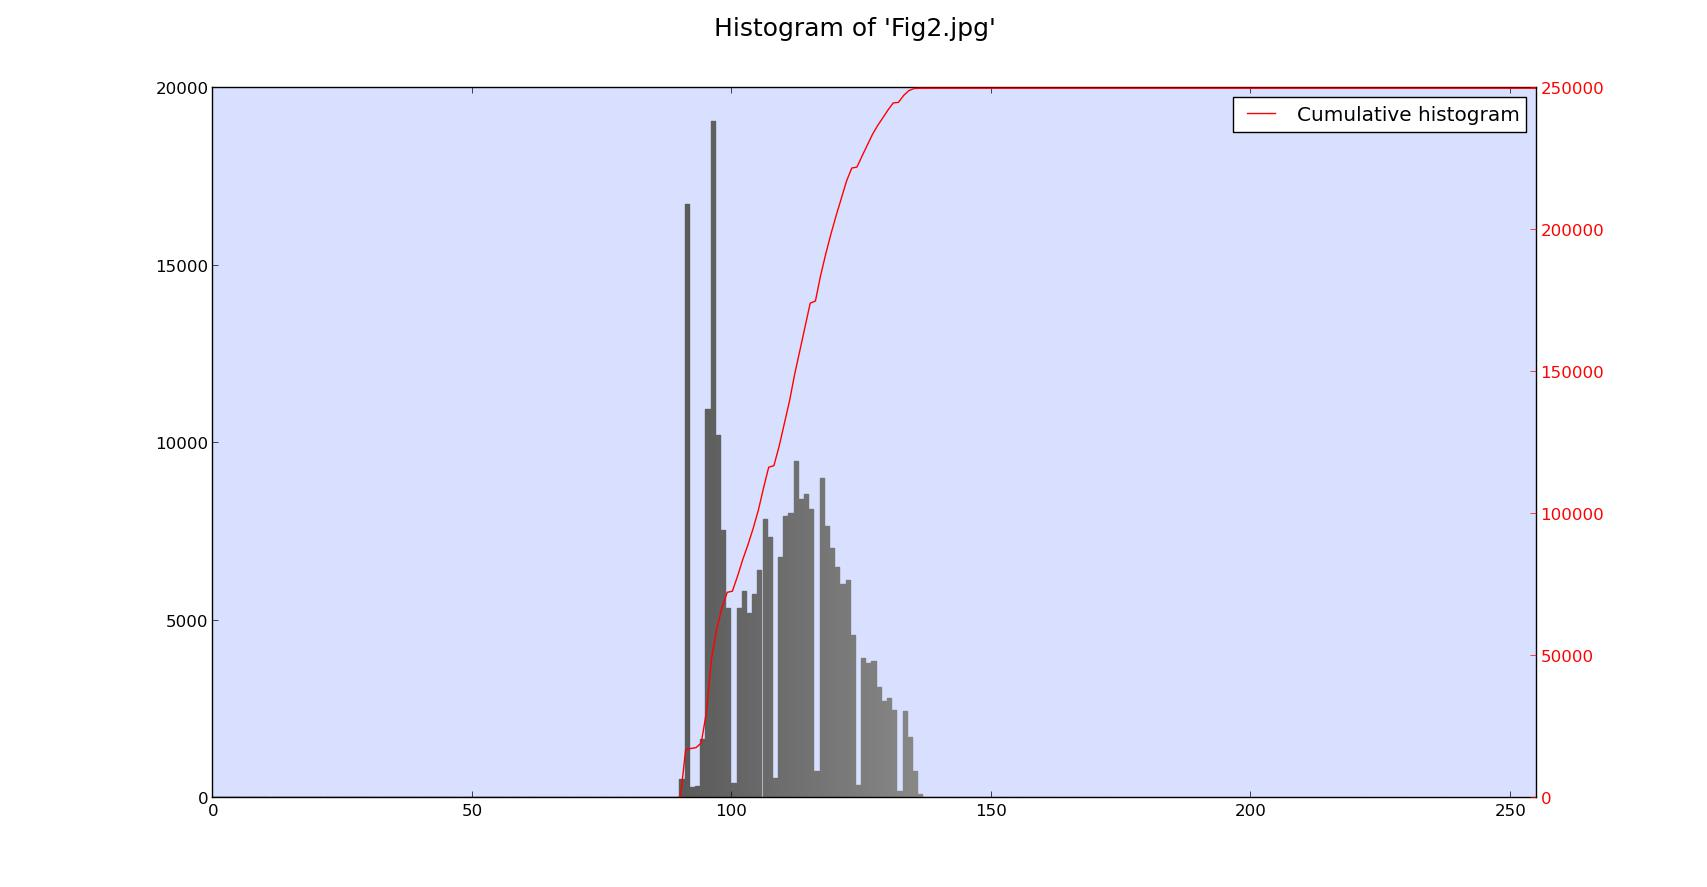
\includegraphics[width=\linewidth]{./images/Histogram_Fig2.jpg}
        \caption{Histogram of "Fig1.jpg"}
        \label{diagram:hist_fig2}
    \end{figure}

    \subsection{Histogram equalization}

    \begin{figure}[h]
        \centering
        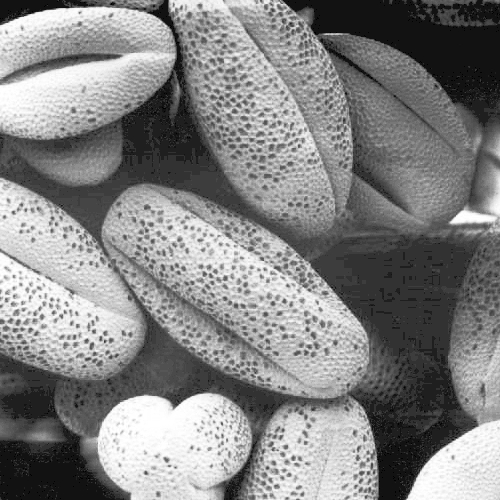
\includegraphics[width=\linewidth]{./images/Enhanced_Fig2.jpg}
        \caption{Enhanced "Fig2.jpg"}
        \label{diagram:enhanced_fig2}
    \end{figure}

    \begin{figure}[h]
        \centering
        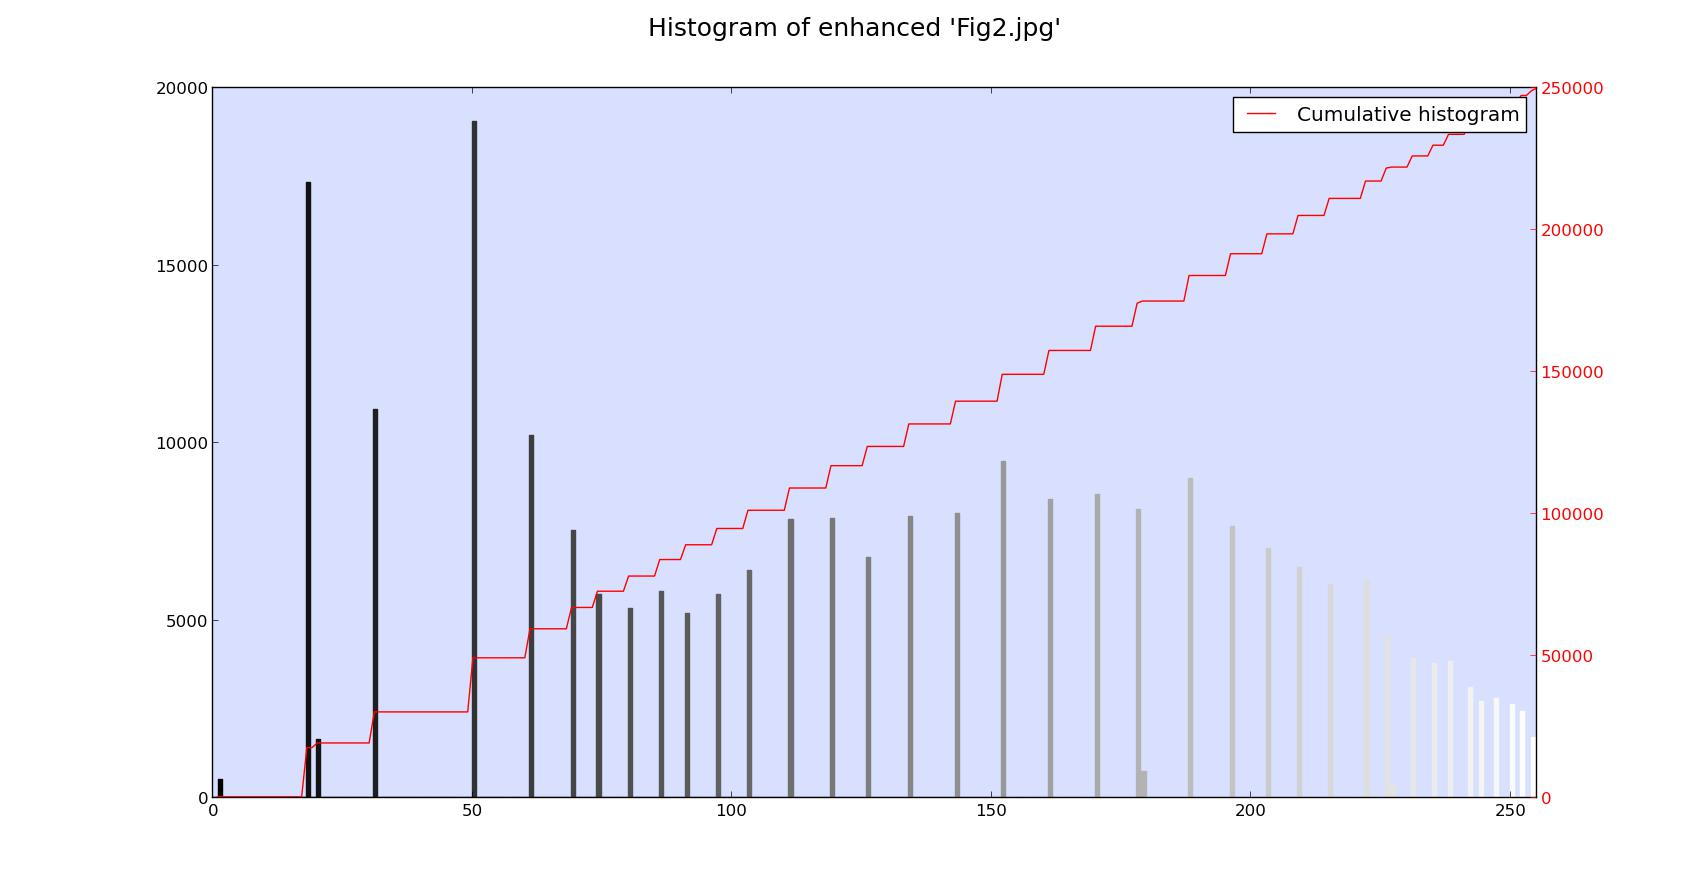
\includegraphics[width=\linewidth]{./images/Equalized_Histogram_Fig2.jpg}
        \caption{Equalized histogram of "Fig2.jpg"}
        \label{diagram:equal_hist_fig2}
    \end{figure}
